% !TEX root = ../main.tex
% Chapter 3

\chapter{Change detection by Support Vector Machines}

\label{Chapter3} % For referencing the chapter elsewhere, use \ref{Chapter3}

\lhead{Chapter 3. \emph{Change detection by Support Vector Machines}} % This is for the header on each page - perhaps a shortened title

%----------------------------------------------------------------------------------------
\section{Outline}
\emph{Not intented for the reader.}
\begin{itemize}
  \item Content follows blogpost, but more formal
  \item Explain the connection between change detection and \{outlier detection, density estimation, \etc\}
  \item Explain change detection in relation with ``M-Estimators''.
  \item Explain why and how SVM can be used for outlier detection, and thus for change detection in time series
  \item Explain options when using SVM, such as RBF kernel
  \item Relate characteristics of (accelerometer) data to the used (RBF?) kernel
  \item Define some quality metrics --> this should be in a different chapter (About experiments)
  \item Note: try to avoid the perspective of \emph{density estimation}. Instead: \emph{data description} or \emph{boundary description}.
\end{itemize}

This chapter discusses the concepts and algorithms that will be used as a basis for the proposed method, as discussed in Chapter \ref{Chapter4}.
The first sections formulates the problem of change detection and relates it to outlier and novelty detection.
It transforms the traditional problem to change detection for times series data.
In Section \ref{sec:one_class_classification} the problem of \acrlong{occ} is discussed and shows a number of implementations.
Two \acrlong{svm}-based methods, \gls{nu-svm} and \gls{svdd}, are further disussed in section \ref{sec:one_class_svm}.
\TODO{add \ref{sec:svm_parameters}}
For the application to the problem of \acrlong{har}, the characteristics of the collected sensor data is discussed in \ref{sec:sensor_data_characteristics}.
Finally a theoretic set of quality metrics is discussed in Section \ref{sec:quality_metrics}.

% !TEX root = ../../main.tex
\section{Change Detection in Time Series}\label{sec:change_detection_time_series}
\TODO{Write section introduction} \\
\emph{The section should relate the problem of outlier detection to change detection.
It should transform the traditional problem formulation to that of time series data.
Build to one-class classification, which can be used for outlier detection}

\subsection{Relation to outlier detection}
The problems of outlier and novelty detection, segmentation, and change detection are closely related.
The terminology depends on the field of application, but there are subtle differences.
The problem of outlier detection is concerned with finding data objects in a data set which have small resemblance with the majority of the data objects.
These objects can be regarded as erroneous measurements.
In the case of novelty detection these objects are considered to be member of a new class of objects.
The unifying framework of Takeuchi and Yamanishi \cite{takeuchi2006unifying}, \gls{changeFinder}, creates a two stage process expressing change detection in terms of outlier detection.
The first stage determines the outliers in a time series by giving a score based on the deviation from a learned model, and thereby creates a new time series.
The second stage runs on that new created time series and calculates a average over a window of the outlier scores.
The problem of change detection is then reduced to outlier detection over that average-scored time series.
The implementation by Camci \cite{camci2010change}, \gls{svcpd}, implements outlier detection with the \gls{svdd} algorithm to detect changes in mean and variance.

\subsection{Problem formulation}\label{subsec:change_detection_problem_formulation}
\TODO{Note: the following block is copied from~\ref{sec:method_change_indication}} \\
The problem of change point detection can be formulated using different type of models, as discussed in~\ref{subsec:segmentation}.
The methods by Takeuchi and Yamanishi \cite{takeuchi2006unifying} and Camci \cite{camci2010change} use the following formulation for change detection, which we will also use for our problem formulation.
The algorithm searches for sudden changes in the time series data.
In other words, slowly changing properties in the data are not considered to be changes.
Considered a time series $x_1 x_1 \dots$, which is drawn from a stochastic process $p$.
Each $x_t$ (t = 1, 2, \dots) is a $d$-dimensional real valued vector and $p$ a probability density function of the sequence $x_1 x_2 \dots$.
Assume $p$ can be decomposed in two different \gls{iid} stationary stochastic processes $p^1$ and $p^2$ and are one-dimensional Gaussian density functions.
For a time point $a$ data points for which $t < a$ are drawn from $p^1 = N(\mu_1, \sigma_1^2)$ and for $t \geq a$ from $p^2 = N(\mu_2, \sigma_a^2)$.
If $p^1$ and $p^2$ are different, then the time point $t = a$ is a \emph{change point}.
In \cite{takeuchi2006unifying} the similarity between the stochastic processes are expressed by the \gls{kl} divergence $D(p^2||p^1)$.
It is observed that this measure is not able to detect a change by decrease in variance \cite{takeuchi2006unifying,camci2010change}.
This problem is the motivation for Camci \cite{camci2010change} to create the \gls{svcpd} algorithm.

The definition of change point being sudden changes in the time series data is in line with the search of changes in activities.
Since we are only interested in different activities (which are represented by sudden changes), slight changes within an activity are not of interest.
\Cref{sec:sensor_data_characteristics} discusses the representation of activities and changes between them in the data in more detail.

\TODO{add more formal definition or analysis of change detection}

-- Literature --

``Online segmentation of time series based on polynomial least-squares approximations'', \cite{fuchs2010online}. 25, 2010 \\

% \subsection{General framework for outlier detection}
% In \cite{schubert2012local} a general framework for outlier detection is proposed.
% The authors compare existing methods and identified the common building block of the algorithms.
% The focus is on unsupervised methods, using information from a local selection of data objects for the detection of outliers.
% The following common algorithmic building blocks are identified:

% \begin{enumerate}
%   \item Context: a ``local'' context of an object $o$ for model building
%   \item Model: the method used for building the model
%   \item Reference: a ``reference'' context of object $o$ for model comparison
%   \item Comparison: the method used for model comparison
%   \item Normalization: a (global) normalization procedure
% \end{enumerate}

% Here the \emph{context} and \emph{reference} are sets of objects used for model building and model comparison, respectively.


% \subsection{Regression, Classification, etc}

% General framework of outlier detection, change detection in context of (simple?) regression, classification.

% \subsection{M-estimators}
% \TODO{Move this section to somewhere in the end; is specification/extension, not base material}
% To make a method less sensitive to outliers (in the training data) techniques from robust statistics are applied.
% The term \emph{robustness} has many interpretations, one of them that it ``signifies insensi­tivity to small deviations from the [prior] assumptions [about the underlying situation]'', according to Huber \cite{huber2009robust}.
% Methods have been proposed to apply robust statistics in the form of M-estimators to \glspl{svm}, such as \cite{choi2009least,chen2004m,suykens1999least}.

% \TODO{Question: do slack-variables (allowance of outliers) make SVM robust?}
% !TEX root = ../../main.tex
\section{One-Class Classification}\label{sec:one_class_classification}
As discussed in the previous section, change detection in time series can be implemented using outlier, or novelty, detection.
To regard a data point as an outlier, there must be a model of the normal time series data and a (dis)similiarity measure defined over the model and data objects.
When a data point differs enough from the created model, it can be labeled as an outlier.
The class of \gls{occ} algorithms is especially designed for that purpose.
The algorithms build up a model of the data, assuming only normal data objects are available (or a very limited amount of example outlier data objects).
This is also known as novelty detection or semi-supervised detection and is of Type 3 in the system by Hodge and Austin~\cite{hodge2004survey}.
This differs from classical classification algorithms, which commonly rely of both positive and negative examples.

In \Cref{subsec:occ-problem-formulation} the problem formulation of \gls{occ} methods is explained.
In \cref{subsec:occ-methods} an overview of \gls{occ} methods is given.
The following section will discuss one specific set of methods, the \gls{oc-svm} which use \glspl{svm} to model the normal training data.

\subsection{Problem formulation}\label{subsec:occ-problem-formulation}
The problem of \acrlong{occ} is closely related to the (traditional) two-class classification situation\footnote{Two-class problems are considered the basic problem, since multi-class classification problems can be decomposed into multiple two-class problems \cite{fukunaga1990introduction}.}.
In the case of traditional classification algorithms, the problem is to assign an unknown object to one of the pre-defined categories.
Every object $i$ is represented as a d-dimensional vector $\vectorsym{x}_i = (x_{i,1},\dots,x_{i,d}), x_{i,j} \in \mathbb{R}$.
Using this notation, an object $\vectorsym{x}_i$ thus represents one point in a feature space $\mathcal{X} \in \mathbb{R}^d$.
The two classes of objects, $\omega_1$ and $\omega_2$, are labeled $-1$ and $+1$ respectively.
The objects with a label $y_i \in \{-1, +1\}$ are in the training set (note that it can be both positive and negative example objects).
This problem is solved by determining a decision boundary in the feature space of the data objects and label the new data object based on the location relative to this boundary.
This is expressed by the decision function $y = f(\vectorsym{x})$:
\begin{equation}\label{eq:decision_function_classification}
  f: \mathbb{R}^d \rightarrow \{-1, +1\}
\end{equation}
In case of the \gls{occ} problem, only one class (often referred as the target class, or positive examples) of training data is used to create a decision boundary.
The goal is to determine whether a new data object belongs to the target class.
If it does not belong to the class it is an outlier.
One could argue that this problem is equal to the traditional two-class problem by considering all other classes as negative examples, although there are important differences.
In pure \gls{occ} problems there are no negative example objects available.
This could be because the acquisition of these examples is very expensive, or because there are only examples of the `normal' state of the system and the goal is to detect `abnormal' states.
Since the algorithm's goal is to differentiate between normal and abnormal objects (relative to the training objects), \gls{occ} is often called outlier, novelty or anomaly detection, depending on the origin of the problem to which the algorithm is applied\footnote{The term \acrlong{occ} originates from Moya \etal \cite{moya1993one}.}.
The difference between two and one-class classification and the consequence for outlier objects is illustrated in \Cref{fig:two-vs-one-classification}.
In the two-class classification problem the object \textbf{o} will be member of the \textbf{-1} class whilst the \gls{occ} problem will label it as an outlier.
In \cite{tax2001one} a more detailed analysis of the \gls{occ} is given.

\begin{figure}
  \centering
    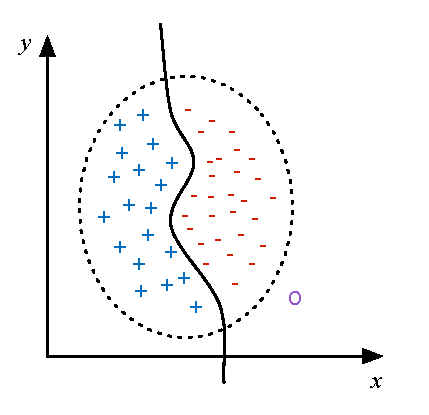
\includegraphics[width=0.5\textwidth,keepaspectratio]{./Figures/chapter3/two-vs-one-classification.pdf}
  \caption[Difference between two and one-class classification]{This plot shows the difference between two and one-class classification. The solid line indicates a possible decision boundary between the \textbf{+1} and \textbf{-1} example objects. The dashed circle indicates the closed boundary around all the data objects. In the first type the object \textbf{o} is considered to be member of the \textbf{-1}-class, whilst in the latter (\gls{occ}) formulation it is an outlier.}
  \label{fig:two-vs-one-classification}
\end{figure}

The \gls{occ} algorithms have been applied to a wide range of applications.
The first is, obviously, outlier detection of objects which do not resemble the bulk of the training data.
It can be a goal by itself and can be used as a filtering mechanism for other data processing methods.
Often methods that rely on data characteristics are sensitive for remote regions in the data set.
Using \gls{occ} these remote regions can be removed from the data set.
A second application is for the problem as described above, in which only data from a single target class is available.
When this problems originates from \eg a monitoring process, the \gls{occ} is able to recognize abnormal system states, without the need to create (or simulate) faulty states beforehand.
The final possible application given by Tax \cite{tax2001one} is the comparison of two data sets.
By constructing a \gls{occ}-classifier using a training data set, one can compare that set to a new data set.
This will result in a similarity measure expressed in the properties of outliers.
This is related to other methods of expressing similarity, such as density-ratio estimation and the \gls{kl} divergence as discussed in \Cref{sec:change_detection_time_series}.

\subsection{One-Class Classification methods}\label{subsec:occ-methods}
The methods and algorithms used for the \gls{occ}-problem can be organized into three categories \cite{tax2001one,noumir2012simple}, visually represented in \Cref{fig:occ-methods}.
The first category consists of methods that estimate the density of the training data and set a threshold on this density.
Among those are Gaussian models, \glspl{gmm} and Parzen density estimators.
In order to get good generalization results with these methods, the dimensionality of the data and the complexity of the density need to be restricted.
This can cause a large bias on the data.
When a good probability model is postulated, these methods work very well. %, since when one threshold is optimized, a minimum volume is automatically found for the given probability density model \cite{tax2001one}.

Boundary methods are based on Vapnik's principle\footnote{With a limited amount of data available, one should avoid solving a more general problem as an intermediate step to solve the original problem \cite{vapnik1998statistical}.} which imply in this case that estimating the complete data density for a \gls{occ} may be too complex, if one is only interested in the closed boundary.
Examples of methods that focus on the boundary (a direct threshold) of the training data distribution are K-centers, Nearest-neighborhood, and \gls{svdd}, or a combination of those methods \cite{hempstalk2008one}.
Especially \gls{svdd} has a strong bias towards minimal volume solutions.
These type of methods are sensitive to the scale and range of features, since they rely on a well-defined distance measure.
The number of objects that is required, is smaller than in the case of density methods.
The boundary method \gls{svdd}, constructed by Tax and which has shown good performance \cite{khan2010survey}, will be further discussed in \Cref{subsec:oc-svm-svdd}.

Reconstruction methods take a different approach.
Instead of focusing on classification of the data and thus on the discriminating features of data objects, they model the data.
This results in a compact representation of the target data and for any object a reconstruction error can be defined.
Outliers are data objects with a high error, since they are not well reconstructed by the model.
Examples of reconstruction methods are K-means, \gls{pca} and different kind of neural network implementations.

\begin{figure}
  \centering
    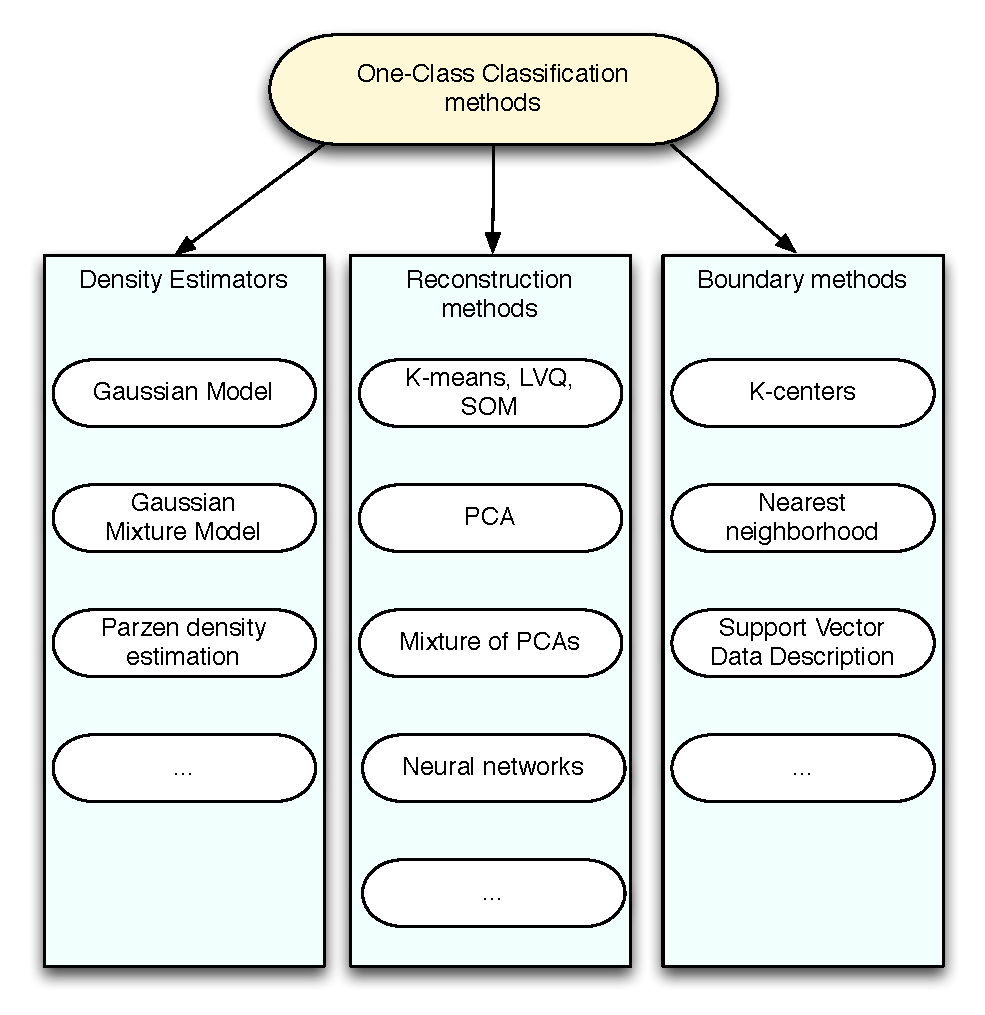
\includegraphics[width=0.5\textwidth,keepaspectratio]{./Figures/chapter3/occ_methods.pdf}
  \caption[\gls{occ} methods]{Overview of \gls{occ} methods categorized in Density Estimation, Reconstruction methods, and Boundary methods. This categorization follows the definition of Tax in \cite{tax2001one}.}
  \label{fig:occ-methods}
\end{figure}

In \cite{khan2010survey,noumir2012simple} an overview of applications for \gls{occ}-algorithms, and explictly for \gls{svm}-based methods (such as \gls{svdd} and \gls{nu-svm}), is given.
It shows succesful applications for, amonst others, problems in the field of Handwritten Digit Recognition, Face Recognition Applications, Spam Detection and Anomaly Detection \cite{li2003improving,perdisci2006using}.
As discussed in \Cref{sec:change_detection_time_series}, this can be used for change detection in time series data.

In this Section we have discussed the problem of \gls{occ} and different kind of implementations.
An often used implementation is the \gls{svm}-based method \cite{noumir2012simple}, since is shows good performance in comparitive researches \cite{khan2010survey,smola1998connection}.
In the following section (\ref{sec:one_class_svm}) two implementations of \gls{oc-svm} will be discussed, the \gls{svdd} method of Tax and Duin \cite{tax1999support} and the \gls{nu-svm}-algoritm by Sch\"olkopf.

% -- Literature --

% ``A survey of recent trends in one class classification'' \cite{khan2010survey}. 25, 2010 \\

% ``One-class classification by combining density and class probability estimation'' \cite{hempstalk2008one}. 51, 2008 \\

% ``One-class classification'' \cite{tax2001one}. 693, 2001 \\

% ``The One-Class Classification Approach to Data Description and to Models Applicability Domain'' \cite{baskin2010one}. 19, 2009 \\

% ``One-class classifier networks for target recognition applications'' \cite{moya1993one}. 70, 1993. Origin of term ``One-Class Classification'' \\
% !TEX root = ../../main.tex
\section{One-Class Support Vector Machine}\label{sec:one_class_svm}
In this section we will discuss the details of an \gls{svm} and \gls{oc-svm} implementations.
The classical implementation of an \gls{svm} is to classify a dataset in two distinct classes.
This is a common use case, although sometimes there is no training data for both classes available.
Still, one would like to classify new data points as regular, in-class, or out-of-class, \eg in the case of a novelty detection.
With that problem only data examples from one class are available and the objective is to recognize new data points that are not part of that class.
This unsupervised learning problem is closely related to density estimation.
In that context, the problem can be the following.
Assume an underlying probability distribution $P$ and a data point $\vectorsym{x}$ drawn from this distribution.
The goal is to find a subset $S$ of the input space, such that the probability that $\vectorsym{x}$ lies inside of $S$ equals some predetermined value $\nu$ between $0$ and $1$ \cite{scholkopf1999support}.

In the following of this section we will start with a discussion of traditional \glspl{svm}.
In \Cref{subsec:kernels} we will show how kernels allow for non-linear decision functions.
That is followed by two different implementations of \gls{oc-svm}: \gls{nu-svm} in \Cref{subsec:nu-svm} by Sch\"olkopf \etal \cite{scholkopf1999support}, which closely follows the above problem statement regarding density estimation, and \gls{svdd} by Tax and Duin \cite{tax1999support} in \Cref{subsec:oc-svm-svdd}.
The final part of this section discusses the influence of model parameters on the performance of \glspl{svm}

%--------------------------------------------
\subsection{Support Vector Machine}\label{subsec:svm}
We will first discuss the traditional two-class \gls{svm} before we consider the one-class variant, as introduced by Cortes and Vapnik in \cite{cortes1995support}.
Consider a labeled data set $\Omega = \{ (x_1, y_1),\allowbreak (x_2, y_2), \dots , (x_n, y_n) \}$; points $x_i \in \mathbb{I}$ in a (for instance two-dimensional) space where $x_i$ is the $i$-th input data point and $y_i \in \{-1, 1\}$ is the $i$-th output value, indicating the class membership.

An \gls{svm} can create a boundary between linear-separable data points, making it a binary linear classifier.
More flexible non-linear boundaries can be obtained by the use of a non-linear function $\phi(x)$, as illustrated in \Cref{fig:kernel_mapping}.
This function maps the input data from space $\mathcal{I}$ to a higher dimensional space $\mathcal{F}$.
The \gls{svm} can create a linear separating hyperplane in the space $\mathcal{F}$ that separates the data points from the two classes.
When the hyperplane is projected on to the (lower) original input space $\mathcal{I}$ it creates a non-linear separating curve.
A schematic overview of this process is illustrated in \Cref{fig:svm_mapping_spaces}.
The original data points $x \in \mathcal{I}$ are projected by $\phi(x)$ to the points $z \in \mathcal{F}$.
In that space the linear hyperplane is constructed by weights $w$.
This results in a non-linear hyperplane $y$ in input space $\mathcal{I}$.
The mapping and projection of data points can be efficient (and implicit) performed by using the kernel trick, which is discussed in \Cref{subsec:kernels}.

\begin{figure}
\centering
  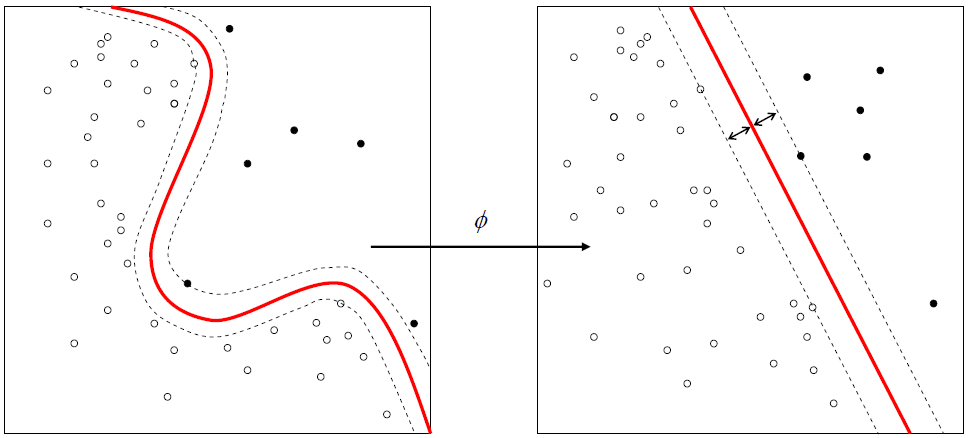
\includegraphics[width=0.8\textwidth]{./Figures/chapter3/svm_kernel_mapping.png}
  \caption[Kernel mapping]{Visualization of an \gls{svm} in 2D.
  The non-linear boundary in the input space $\mathcal{I}$ (left) is transformed to a linear boundary in the feature space $\mathcal{F}$ (right) by mapping the data points with the function $\phi$.
  The kernel trick uses a function $K$ which performs an implicit mapping. Image from Wikipedia.org}
  \label{fig:kernel_mapping}
\end{figure}

\begin{figure}
\centering
  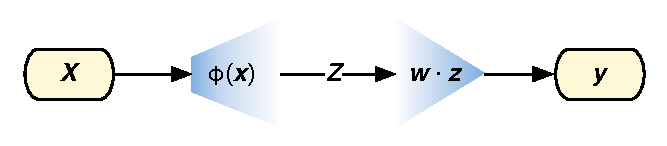
\includegraphics[width=0.8\textwidth]{./Figures/chapter3/svm_mapping_spaces.pdf}
  \caption[Mapping spaces in \gls{svm}]{Schematic visualization of the non-linear mapping of \glspl{svm}.
  The input vector $\vectorsym{x}$ from input space $\mathcal{I}$ is mapped by a non-linear function $\phi(\vectorsym{x})$ to a feature vector $\vectorsym{z}$ in the high dimensional feature space $\mathcal{F}$.
  The weights of $\vectorsym{w}$ create a linear separating hyperplane, which maps the high dimensional vector to the predicted outcome $\vectorsym{y}$.}
  \label{fig:svm_mapping_spaces}
\end{figure}

The separating hyperplane is represented by
\begin{equation}
w^T x + b = 0,
\end{equation}
with $w \in \mathcal{F}$ and $b \in \mathbb{R}$.
The hyperplane that is created determines the \emph{margin} between the classes; the minimal distance from the data points to the hyperplane.
In geometric sense, $w$ is the normal vector indicating the direction of the hyperplane and $\frac{b}{\lVert{w}\rVert}$ determines the offset of the hyperplane from the origin.
Since the size of the margin is equal to $\frac{2}{\lVert{w}\rVert}$, the maximum-margin hyperplane is found by minimizing $\lVert{w}\rVert$.
The data points which lie on the boundary of the margin are the \emph{support vectors}.
This geometrical interpretation is illustrated in \Cref{fig:svm_hyperplane}.
All data points for which $y_i = -1$ are on one side of the hyperplane and all other data points (for which $y_i = 1$) are on the other side.
The minimal distance from a data point to the hyperplane is equal for both classes.
Minimizing $\lVert{w}\rVert$ results in a \emph{maximal margin} between the two classes.
Thus, the \gls{svm} searches for a maximal separating hyperplane.

\begin{figure}
\centering
  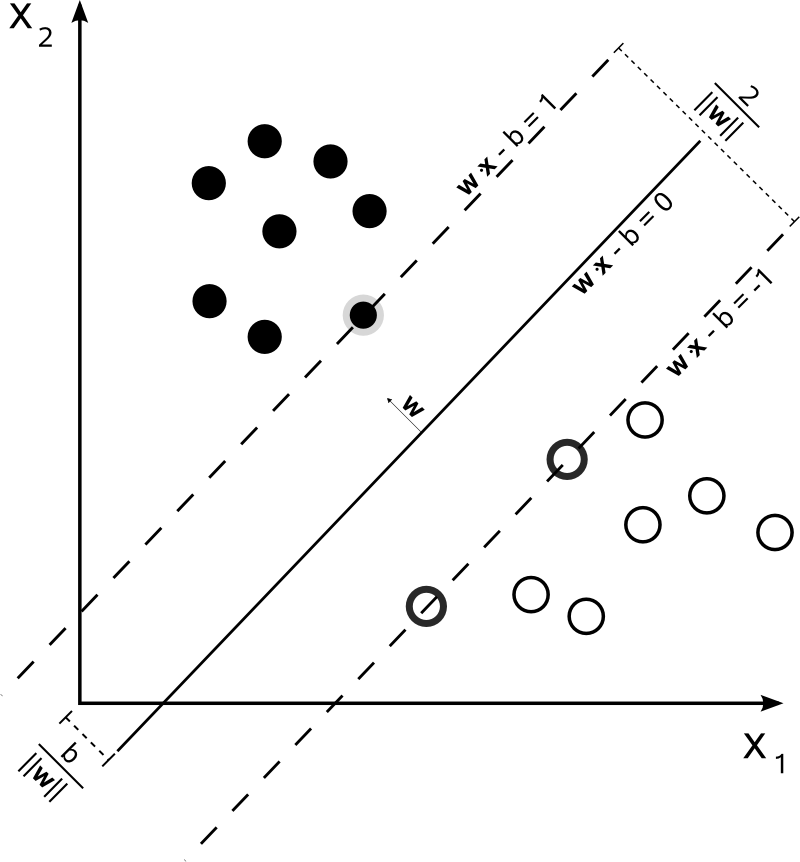
\includegraphics[width=0.5\textwidth]{./Figures/chapter3/svm_separating_plane_with_margin.png}
  \caption[\gls{svm} and the separating hyperplane]{Illustration of the separating hyperplane of an \gls{svm}.
  Here $w$ is the normal vector for the separating hyperplane and size of the margin is $\frac{2}{\lVert{w}\rVert}$.
  Image from Wikipedia.org}
  \label{fig:svm_hyperplane}
\end{figure}

With every classification method there is a risk of overfitting.
In that case the random error or noise of the data set is described instead of the underlying data.
The \gls{svm} classifier can use a \emph{soft margin} by allowing some data points to lie within the margin, instead of on the margin or farther away from the hyperplane.
For this it introduces \emph{slack variables} $\xi_i$ for each data point and the constant $C > 0$ determines the trade-off between maximizing the margin and the number of data points within that margin (and thus the training errors).
The slack variables are a generalization to minimize the \emph{sum of deviations}, rather than the \emph{number} of incorrect data points \cite{cherkassky2007learning}\footnote{if $\xi_i$ is chosen to be an indicator function, it still minimizes the \emph{number} of incorrect data points.}.
The objective function for an \gls{svm} is the following minimization function:

\begin{equation}\label{eq:svm_objective}
  \operatorname*{min}_{w,\ b,\ \xi_i} \frac{ \lVert{w}\rVert^2 }{2} + C \sum_{i=1}^n \xi_i
\end{equation}
\begin{equation}
  \begin{multlined}
  \mbox{ subject to: } \\*
  \begin{aligned}
  y_i( w^T \phi(x_i) + b) \geq \: & 1 - \xi_i & \mbox{ for all } i = 1, \dots, n \\*
   & \xi_i \geq 0 & \mbox{ for all } i = 1, \dots, n\\*
  \end{aligned}
  \end{multlined}
\end{equation}

This minimization problem can be solved (using \gls{qp}) and transformed to its (Lagrange) dual formulation.
In the dual formulation the problem scales with the number of training examples $n$ instead of the dimensionality $d$ of the samples.
Solving this problem directly in the high dimensional feature space $\mathcal{F}$ makes it intractable.
The linear approximation function corresponds to the kernel function in the dual formulation.
Solving this dual formulation is equivalent to solving the primal formulation \cite{cherkassky2007learning}.
In the dual formulation the Lagrange multipliers $a_i >= 0$ are introduced and the decision function becomes:
\begin{equation}\label{eq:svm_lagrange}
  f(x) = \operatorname{sgn}( \sum_{i=1}^n \alpha_i y_i K(x, x_i) + b),
\end{equation}
where $K(x, x_i) = \phi(x)^T\phi(x_i)$ is the dot product of data objects in feature space $\mathcal{F}$ (which is further discussed in \Cref{subsec:kernels}).
Here every data point in $\mathcal{I}$ for which $a_i > 0$ is weighted in the decision function and thus ``supports'' the classification machine: hence the name ``\acrlong{svm}''.
Since it is shown that under certain circumstances \glspl{svm} show an equality to sparse representations \cite{girosi1998equivalence,smola1998connection}, there will often be relatively few Lagrange multipliers with a non-zero value.

Using this formulation two important properties arise \cite{flach2012machine}:
\begin{enumerate}
  \item Searching for the maximum margin decision boundary is equivalent to searching for the support vectors; they are the training examples with non-zero Lagrange multipliers.
  \item The optimization problem is entirely defined by pairwise dot products between training examples: the entries of the kernel matrix $K$.
\end{enumerate}
An effect of the first property, combined with the equality to sparse representations, is that \glspl{svm} often have good results, even in the case of high dimensional data or limited training examples \cite{cherkassky2007learning}.
The second property is what enables an powerful adaptation of \glspl{svm} to learn non-linear decision boundaries.
The workings of the kernel matrix $K$ and the non-linear boundaries are discussed in the following section.

%--------------------------------------------

\subsection{Kernels}\label{subsec:kernels}
In the previous section, the mapping function $\phi(x)$ and the kernel function $K$ were briefly mentioned.
The decision function in \Cref{eq:svm_lagrange} only relies on the dot products of mapped data points in the feature space $\mathcal{F}$ (\ie all pairwise distances between the data points in that space).
It shows \cite{flach2012machine} that for any function $K$ that has the same result in feature space $\mathcal{F}$, without an explicit mapping to the higher dimension $\mathcal{F}$, the dot products can be substituted by the kernel function $K$, as introduced by Aizerman~\etal \cite{aizerman1964theoretical} and applied to \glspl{svc} by Vapnik \cite{vapnik1998statistical}:
\begin{equation}
  K(\vectorsym{x}, \vectorsym{x}') = (\vectorsym{z} \cdot \vectorsym{z}') = \phi(\vectorsym{x}) \cdot \phi(\vectorsym{x}')
\end{equation}
where vectors $\vectorsym{z}$ and $\vectorsym{z}'$ are projections of data objects $\vectorsym{x}$ and $\vectorsym{x}'$ through $\phi(\vectorsym{x})$ on the features space $\mathcal{F}$.
The dot product kernel $K$ is determined by the sum
\begin{equation}
  K(\vectorsym{x}, \vectorsym{x}') = \sum_{j=1}^m g_j(\vectorsym{x}) g_j(\vectorsym{x}')
\end{equation}
of basis functions $g_j(\vectorsym{x})$.
Note that the evaluation of dot products in the feature space $\mathcal{F}$ between vectors is performed indirectly via the evaluation of the kernel $K$ between (support) vectors in the input space $\mathcal{I}$.
This is known as the \emph{kernel trick} and gives the \gls{svm} the ability to create non-linear decision function without high computational complexity.

The kernel function $K$ can have different forms, such as linear, polynomial and sigmoidal but the most used (and flexible) form is the Gaussian \gls{rbf}.
The basis functions have the form
\begin{equation}
  g(x) = \operatorname*{sign} \left(  \sum_{i=1}^{n} \alpha_i \operatorname*{exp} \left\{ \frac{\rVert \vectorsym{x} - \vectorsym{x}_i \rVert ^2}{\sigma^2} \right\} \right),
\end{equation}
where $\sigma$ defines the width and $\rVert \vectorsym{x} - \vectorsym{x}' \rVert ^2$ is the dissimilarity measure expressed as Euclidian distance.
The inner product kernel $K$ then becomes
\begin{equation}
  K(\vectorsym{x}, \vectorsym{x}') = \operatorname*{exp} \left\{ - \frac{ \rVert \vectorsym{x} - \vectorsym{x}' \rVert ^2}{\sigma^2} \right\}.
\end{equation}
The kernel $K$ maps input space $\mathcal{I}$ to the feature space $\mathcal{F}$ which is a \gls{rkhs} of (theoretically) infinite dimensions.
As Smola \etal \cite{smola1998connection} state, this Gaussian kernel yields good performance, especially when no assumptions can be made about the data.
As an explanation, they show a correspondence between learning \glspl{svm} with \gls{rbf} kernels and good regularization operators.
This may give insights in why \glspl{svm} have been found to exhibit high generalization ability (by learning with few training objects).

The number of basis functions, the center parameters that correspond with support vectors, and the weights in the output layer are all automatically determined via the optimal hyperplane in features space $\mathcal{F}$ \cite{cherkassky2007learning}.
The width parameter $\sigma$ is equal for all basis functions and is set a priori and determines the flexibility and complexity of the boundary.
In \Cref{subsec:svm_model_parameters} this (hyper)parameter for an \gls{svm} is further discussed.

The mapping from input space $\mathcal{I}$ to $\mathcal{F}$ via $\phi(x)$ is subject to some continuity assumptions.
This general assumption in pattern recognition, states that two near objects in feature space should also resemble each other in ``real life'' \cite{tax2001one}.
Thus, objects which are close in feature space should be close in the original input space.
When this assumption does not hold, the example objects would be scatter through the feature space and finding a decision function becomes very complex.

% -- Quotes and refs to use --x

% sparsity, \gls{rkhs}: \cite{girosi1998equivalence} \\

% Use Chapter 2 from ``Learning with kernels'', \cite{scholkopf2002learning}.

%--------------------------------------------

\subsection{\acrlong{nu-svm}}\label{subsec:nu-svm}
The first of the \gls{oc-svm} methods we will discuss is often referred to as \gls{nu-svm} and introduced by Sch\"olkopf \etal \cite{scholkopf1999support}.
Instead of estimating the density function of an distribution $P$, it focuses on an easier problem: the algorithm finds regions in the input where the ``probability density lives''.
This results in a function such that most of the data is in the region where the function is nonzero.

The constructed decision function $f(x)$ resembles the function discussed in \Cref{subsec:svm}.
It returns the value $+1$ in a (possibly small) region capturing most of the data points, and $-1$ elsewhere.
The method maps the data points from input space $\mathcal{I}$ to a feature space $\mathcal{F}$ (following classical \glspl{svm}).
In that space the data points are separated from the origin by a hyperplane, with maximal margin.
Since the mapping to the feature space is based on dot products of the data points, outlier objects (which are dissimilar from the training set) will be closer to the origin.
Thus, maximizing the distance from the hyperplane to the origin increases the discriminating ability of the decision function.
Furthermore, it holds an intuitive relationship with the classical two-class \gls{svm}.

For a new data points $x$, the function value $f(x)$ determines whether the data point is part of the distribution (\ie the value is $+1$) or a novelty (\ie the value is $-1$).
The hyperplane is represented by $g(x) = w \cdot \phi(x) + \rho = 0$ and the decision function is $f(x) = \operatorname{sgn}(g(x))$.
This hyperplane and the separation from the origin is illustrated in \Cref{fig:nu-svm}.

\begin{figure}
  \centering
    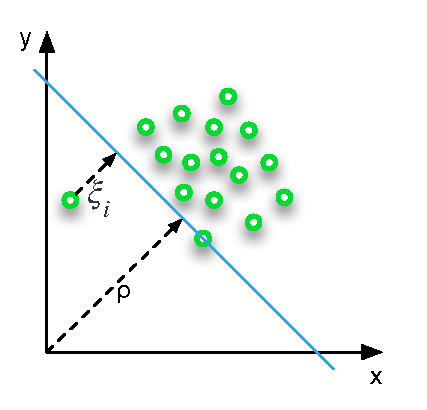
\includegraphics[width=0.5\textwidth,keepaspectratio]{./Figures/chapter3/nu-svm.pdf}
  \caption[\gls{nu-svm}]{Graphical representation of \gls{nu-svm}. The separating hyperplane $w \cdot \phi(x_i) + \rho = 0$ create a maximal margin, in the feature space, between the data points and the origin. Slack variables $\xi_i$ are used to create a soft margin.}
  \label{fig:nu-svm}
\end{figure}

The objective function to find the separating hyperplane is the following minimization function, which can be solved using \gls{qp}:

\begin{equation}\label{eq:nu-svm_objective}
  \operatorname*{min}_{w,\ \xi_i,\ \rho } \frac{\lVert w \rVert ^2}{2} + \frac{1}{\nu n} \sum_{i=1}^n \xi_i - \rho
\end{equation}
\begin{equation}
  \begin{multlined}
    \mbox{ subject to: } \\
    \begin{aligned}
      (w \cdot \phi(x_i)) \geq \: & \rho - \xi_i & \mbox{ for all } i = 1, \dots, n \\
      & \xi_i \geq 0 & \mbox{ for all } i = 1, \dots, n \\
    \end{aligned}
  \end{multlined}
\end{equation}

The decision function in the dual formulation with Lagrange multipliers is denoted as:
\begin{equation}\label{eq:nu-svm_lagrange}
f(x) = \operatorname{sgn}((w \cdot \phi(x_i)) - \rho) = \operatorname{sgn}( \sum_{i=1}^n \alpha_i K(x, x_i) - \rho)
\end{equation}

In the classical \gls{svm} objective function, as denoted in \Cref{eq:svm_objective}, the parameter $C$ decided the smoothness of the boundary, with respect to the slack variables $\xi_i$.
In the formulation of \gls{nu-svm} the equivalent parameter is $\nu \in (0,1)$ (hence the name).
It characterizes the solution in two ways:
\begin{enumerate}
  \item $\nu$ is an upper bound on the fraction of outliers, \ie training examples regarded as out-of-class.
  \item $\nu$ is a lower bound on the fraction of \glspl{sv}, \ie training examples with a nonzero Lagrange multiplier $\alpha_i$.
\end{enumerate}
When $\nu$ approaches $0$, the penalty factor for nonzero Lagrange multipliers ($\frac{1}{\nu n}$) becomes infinite, and thus the solution resembles a \emph{hard margin} boundary.

This method creates a \emph{hyperplane}, characterized by $w$ and $\rho$, that separates the data with maximal margin from the origin in the feature space $\mathcal{F}$.
In the following section we will discuss an alternative method, which uses an circumscribing \emph{hypersphere} to characterize the training data.
The region inside the hypersphere indicates the region $S$ where the probability that a data point drawn from $P$ is equal to $\nu$.


%--------------------------------------------

\subsection{\acrlong{svdd}}\label{subsec:oc-svm-svdd}
The method introduced by Tax and Duin \cite{tax1999support}, known as \acrlong{svdd}, follows a spherical instead of planar approach.
The boundary, created in feature space $\mathcal{F}$, forms a hypersphere around the (high density region of the) data.
The volume of this hypersphere is minimized to get the smallest enclosing boundary.
The chance of accepting outlier objects is thereby also minimized \cite{tax2003online}.
By allowing outliers using slacks variables, in the same manner as classical \gls{svm} and \gls{nu-svm}, a soft margin is constructed.

\begin{figure}
  \centering
    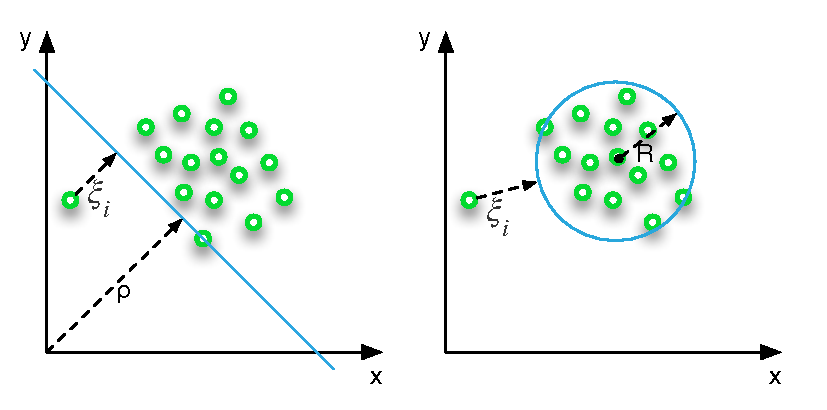
\includegraphics[width=0.8\textwidth,keepaspectratio]{./Figures/chapter3/nu-vs-svdd.pdf}
  \caption[Difference \gls{nu-svm} and \gls{svdd}]{Graphical representation of the difference between \gls{nu-svm} (left) and \gls{svdd} (right). Note that for the sake of simplicity the kernel functions are not applied.}
  \label{fig:nu-vs-svdd}
\end{figure}

The constructed hypersphere is characterized by a center $\mathbf{a}$ and a radius $R > 0$ as distance from the center to (any data point that is a \gls{sv} on) the boundary, for which the volume, and thus the radius $R$, will be minimized.
The center $\mathbf{a}$ is a linear combination of the support vectors.
Like the classical \gls{svm} and \gls{svdd} it can be required that all the distances from the data points $x_i$ to the center $\mathbf{a}$ are strict less than $R$ (or equivalent measure).
A soft margin can be allowed by using slack variables $\xi_i$.
In that case, the penalty is determined by $C$ and the minimization is expressed as \Cref{eq:svdd_objective}.
This principle is illustrated in the right image or \Cref{fig:nu-vs-svdd}.
Instead of a separating hyperplane, constructed by \gls{nu-svm} and illustrated on the left of the Figure, the \gls{svdd} creates a hypersphere (in the illustration a circle) around the data points.
By using kernel functions (\eg the \gls{rbf}) the hyperspheres in the high dimensional feature space $\mathcal{F}$ corresponds to a flexible and tight enclosing boundary in input space $\mathcal{I}$.
Possible resulting closed boundaries are illustrated in \Cref{fig:svdd-boundary}.
This enclosing boundary is obtained by minimizing the following error function $L$ which contains the volume of the hypersphere and the distance from the boundary to the outlier objects:
\begin{equation}\label{eq:svdd_objective}
  L(R, \vectorsym{a}, \vectorsym{\xi}) = R^2 + C \sum_{i=1}^n \xi_i
\end{equation}
\begin{equation}
  \begin{multlined}
    \mbox{ subject to: } \\
    \begin{aligned}
      \lVert x_i - \mathbf{a} \rVert ^ 2 \leq \: & R^2 + \xi_i & \mbox{ for all } i = 1, \dots, n \\
      & \xi_i \geq 0 & \mbox{ for all } i = 1, \dots, n \\
    \end{aligned}
  \end{multlined}
\end{equation}
In the dual Lagrangian formulation of this error function $L$ the multipliers $\vectorsym{\alpha}$ are maximized:
\begin{equation}\label{eq:svdd_lagrange}
  L = \sum_{i} \alpha_i(x_i \cdot x_i) - \sum_{i,j} \alpha_i \alpha_j(x_i \cdot x_j)
\end{equation}
\begin{equation}
  \begin{multlined}
    \mbox{ subject to: } \\
    \begin{aligned}
    0 \le \alpha_i \le C, \: \sum_{i} \alpha_i = 1
    \end{aligned}
  \end{multlined}
\end{equation}

In the maximization of \Cref{eq:svdd_lagrange} a large fraction of the multipliers $\alpha_i$ become zero and for a small fraction $\alpha_i > 0$.
This small fraction, for which $\alpha_i$ is non-zero, are called the \glspl{sv} and these objects lie on the boundary of the description.
The center of the hypersphere only depends on this small number of \glspl{sv} and the objects for which $\alpha_i = 0$ can be discarded from the solution.
Testing the membership of a (new) object $\vectorsym{z}$ is done by determining if the distance to the center $\vectorsym{a}$ of the sphere is equal or smaller to the radius $R$:
\begin{equation}\label{eq:svdd_test_object}
  \lVert \vectorsym{z} - \vectorsym{a} \rVert ^2 = (\vectorsym{z} \cdot \vectorsym{z}) - 2 \sum_{i} \alpha_i(\vectorsym{z} \cdot \vectorsym{x}_i) + \sum_{i,j}(\vectorsym{x}_i \cdot \vectorsym{x}_j) \le R^2
\end{equation}
As with \Cref{eq:svm_lagrange}, the solution of this equation only relies on dot products between the data points in $\vectorsym{x}$ and $\vectorsym{z}$.
This means that the kernel projection and trick, as discussed in \Cref{subsec:kernels}, can be applied to \gls{svdd} as well \cite{tax1999support,tax2002uniform}.

Because the Gaussian \gls{rbf} often yields good (\ie tight) boundaries, this set of kernels functions is commonly used:
\begin{equation}
  (\vectorsym{x} \cdot \vectorsym{y}) \rightarrow K(\vectorsym{x},\vectorsym{y}) = \operatorname{exp}\left(- \frac{\lVert \vectorsym{x} - \vectorsym{y} \rVert ^2}{\sigma^2}\right)
\end{equation}
Using this kernel function, the Lagrangian error function $L$ of \Cref{eq:svdd_lagrange} changes to:
\begin{equation}\label{eq:svdd_lagrange_kernel}
  L = 1 - \sum_{i} \alpha_i^2 - \sum_{i \ne j} \alpha_i \alpha_j K(x_i, x_j)
\end{equation}
Using \Cref{eq:svdd_test_object}, the following kernel formulation needs to hold for a new object $\vectorsym{z}$ to lie within the hypersphere:
\begin{equation}\label{eq:svdd_inequality}
  \sum_{i} \alpha_i K(\vectorsym{z}, x_i) \le \frac{1}{2} \left( 1 - R + \sum_{i,j} \alpha_i \alpha_j K(x_i, x_j) \right)
\end{equation}
When the Gaussian \gls{rbf} kernel is applied, and in case the data is preprocessed to have unit length (for the \gls{nu-svm} solution), the two different \gls{oc-svm} implementations \gls{nu-svm} and \gls{svdd} are shown to have identical solutions \cite{tax2002uniform,scholkopf2002learning}

\begin{figure}
  \centering
    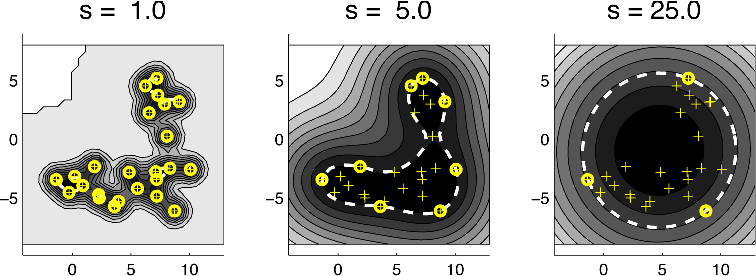
\includegraphics[width=0.5\textwidth,keepaspectratio]{./Figures/chapter3/svdd-boundary.pdf}
  \caption[\gls{svdd} boundary]{The \gls{svdd} method trained on a banana-shaped data set with different sigma-values for the \gls{rbf} kernel. Solid circles are support vectors, the dashed line is the boundary. Image by Tax \cite{tax2001one}.}
  \label{fig:svdd-boundary}
\end{figure}

%--------------------------------------------

\subsection{SVM model parameters}\label{subsec:svm_model_parameters}
\gls{svm}-model selecting and tuning depends on two type of parameters \cite{cherkassky2007learning}:
\begin{enumerate}
  \item Parameters controlling the `margin' size,
  \item Model parameterization, \eg the kernel type and complexity parameters.
  For the \gls{rbf} kernel the width parameter determines the model complexity.
\end{enumerate}

In case of a \gls{rbf} kernel, the width parameter $\sigma$ determines the flexibility and complexity of the boundary.
The value of this parameter greatly determines the outcomes of the algorithm (\eg \gls{svdd}) as illustrated in \Cref{fig:svdd-boundary}.
With a small value for the kernel width $\sigma$, each data point will tend to be used as a support vector (for almost all $\alpha_i > 0$) and the \gls{svdd} solution resembles a Parzen density estimation.
For large values of $\sigma$, the solution will resemble the original hypersphere solution (in contrast with a tight boundary around the data).
With a large value for the width $\sigma$, the boundary approximates the spherical boundary.
The influence of the $\sigma$ parameter on the \gls{svdd} solution is illustrated in \Cref{fig:svdd-boundary-sigma}.

\begin{figure}
  \centering
    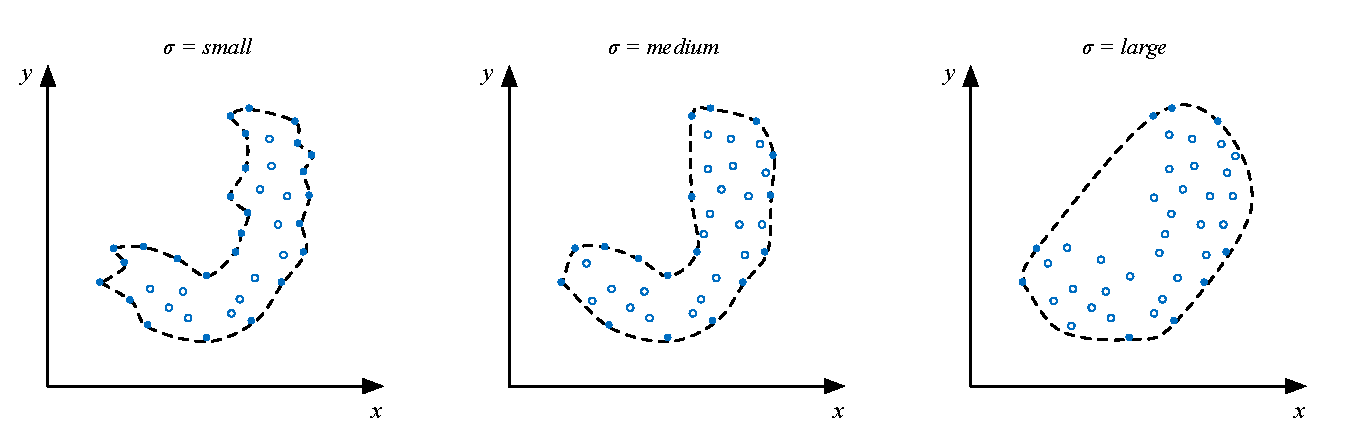
\includegraphics[width=0.8\textwidth,keepaspectratio]{./Figures/chapter3/svdd-parameter-sigma.pdf}
  \caption[\gls{svdd} boundary]{The \gls{svdd} method trained on a banana-shaped data set with different $\sigma$-values for the \gls{rbf} kernel. Solid circles are support vectors, the dashed line is the boundary.}
  \label{fig:svdd-boundary-sigma}
\end{figure}

As discussed in \Cref{subsec:nu-svm}, the \gls{svm} parameter $C$ (or $\nu$ in case of \gls{nu-svm}) is of high influence on the ``smoothness'' of the decision function.
It acts as an upper bound to the fraction of outliers and as a lower bound to the fraction of \glspl{sv}.
A more detailed discussion of the influence of the \gls{svm} model parameters can be found in Section~9.8 of \cite{cherkassky2007learning} and Section~7.4 from \cite{flach2012machine}.
A detailed discussion of the $\nu$ and kernel parameters can be found in \cite{scholkopf2002learning}.

The following chapter will discuss our proposed method, which incorporates the \gls{svdd} algorithm.
It relates the \gls{oc-svm} model construction to outlier detection and eventually change detection, leading to finding a temporal segmentation of time series data.

% -- Notes --
% \begin{itemize}
  % \item Low target rejection rate $f_{T-}$ and low outlier acceptance rate $f_{O+}$. When only target examples are present, the first one can be estimated by the number of support vectors that we obtain as a solution of Lagrangian~\ref{eq:svdd_lagrange_kernel}.
% \end{itemize}

% -- Literature --


% ``A geometric approach to support vector machine (SVM) classification'' \cite{mavroforakis2006geometric}. 136, 2006 \\

% ``Least squares one-class support vector machine'' \cite{choi2009least}. 27, 2009 \\

% ``On simple one-class classification methods'' \cite{noumir2012simple}. 2012  --> decouples radius and center optimization, gives fast approximations instead of precise results. \\

% ``Choosing a small width of the kernels leads to high generalization error as it effectively decouples the separate basis functions of the kernel expansion into very localized functions which is equivalent to memorizing the data, whereas a wide kernel tends to oversmooth.'' \cite{smola1998connection}. \\

% ``For small values of $\sigma$ almost all $\alpha_i >0$ and the \gls{svdd} resembles a Parzen density estimation.'' \cite{tax2002uniform} page 4, \cite{tax1999support} page 4. \\
% !TEX root = ../../main.tex
\section{SVM parameters}\label{sec:svm_parameters}
% !TEX root = ../../main.tex
\section{Sensor data characteristics}\label{sec:sensor_data_characteristics}
\TODO{Other title? More in \acrlong{har} in general?}

-- Literature --
``Sensor-based abnormal human-activity detection'' \cite{yin2008sensor}. 74, 2008 (builds one-class SVM of all normal traces) \\
% !TEX root = ../../main.tex
\section{Quality metrics}\label{sec:quality_metrics}
\TODO{\emph{This section should be in the chapter about experiments}}